\section{Regular expression: complement and intersection}

Regular expressions may also contain the operators of complement, intersection and set difference, which are very useful to make the regexp more concise. 
Let $L$ and $L^{'}$ be regular languages. The complement $\lnot L$ and the intersection$L \cap L^{'}$ are regular languages. The deterministic recognizer $\overline{M}$ 
of the complement language requires to complete the automaton $M$ by adding the error state p and the missing moves: 
\begin{itemize}
    \item Create the error state $p$, not in $Q$, so the states of $\overline{M}$ are $Q \cup \{ p \}$
    \item The transition function $\delta$ is: 
        \begin{itemize}
            \item $\delta(q,a)=\delta(q,a)$, where $\delta(q,a) \in Q$. 
            \item $\delta(q,a)=p$, where $\delta(q,a)$ is not defined;
            \item $\delta(p,a)=p$, for every character $a \in \Sigma$;
        \end{itemize}
    \item Swap the non-final and final states. 
\end{itemize}
\begin{example}
    Find the complement of the given automaton: 
    \begin{figure}[H]
        \centering
        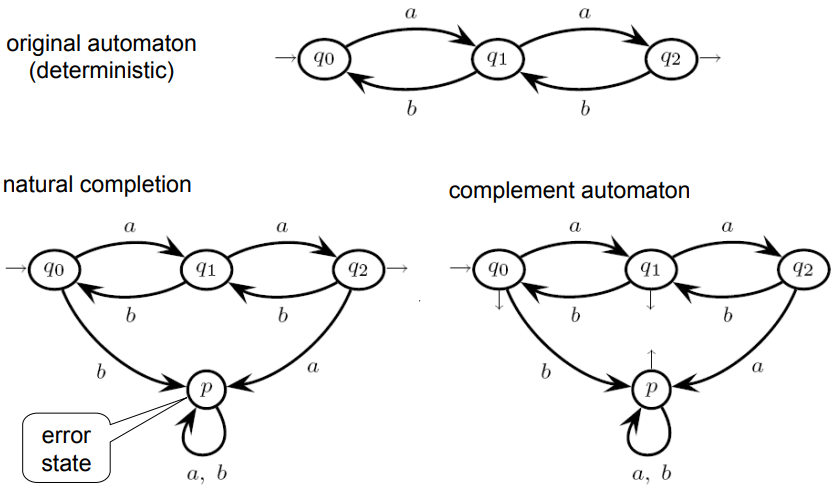
\includegraphics[width=0.8\linewidth]{images/complement.png}
    \end{figure}
\end{example}
For the complement construction to work correctly, the original automaton must be deterministic, otherwise the original and complement languages may be not disjoint,
which fact would be in violation of the complement definition. The complement automaton may contain useless states and may not be in the minimal form either; it should 
be reduced and minimized, if necessary. 
\subsection*{Product of automata}
A very common construction of formal languages, where a single automaton simulates the computation of two automata that work in parallel on the same input string. 
It is very useful to construct the intersection automaton. To obtain the intersection automaton we can resort to the De Morgan theorem. The Cartesian product can 
also be obtained by a more direct construction. The intersection of the two languages is recognized directly by the Cartesian product of their automata. 
Suppose both automata do not contain any spontaneous moves. The state set of the product machine is the Cartesian product of the state sets
of the two automata. Each product state is a pair $\left\langle q^{'},q^{''} \right\rangle $, where the left (right) member is a state of the first (second) machine. 
The move is: 
\[\left\langle q^{'},q^{''} \right\rangle \rightarrow^a \left\langle r^{'},r^{''} \right\rangle \textnormal{ if and only if } q^{'} \rightarrow r^{'} \textnormal{ and } q^{''} \rightarrow r^{''}\]
The product machine has a move if, and only if, the projection of such a move onto the left (right) component is a move of the first (second) automaton. The initial 
and final state sets are the Cartesian products of the initial and final state sets of the two automata, respectively. The product construction is equivalent to simulating both 
machines in parallel.
\begin{example}
    The intersection can be found as follows: 
    \begin{figure}[H]
        \centering
        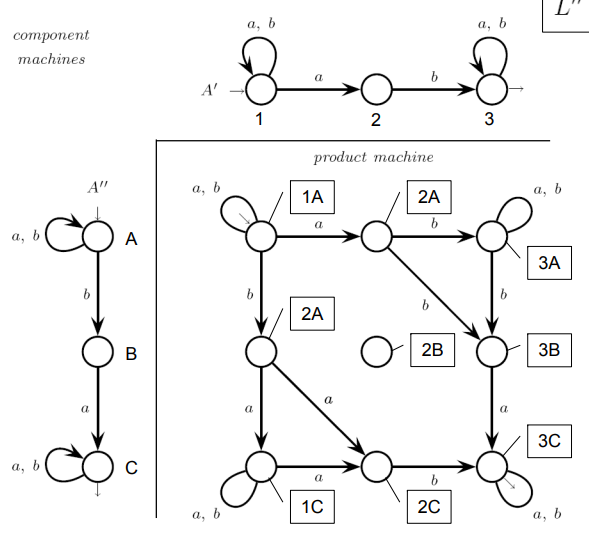
\includegraphics[width=0.52\linewidth]{images/intersection.png}
    \end{figure}
\end{example}